\documentclass{article} % or book or beamer 
\usepackage[utf8]{inputenc}
\usepackage{amsmath}
\usepackage{color}
\usepackage{amssymb}
\usepackage{enumitem}
\usepackage{amsthm}
\usepackage{graphicx}
\usepackage{placeins}
\usepackage{wrapfig}
\usepackage{tikz}
\usepackage{tikz-cd}
\usepackage{chemfig}

\newtheorem{theorem}{Theorem}
\newtheorem{proposition}[theorem]{Proposition}

\theoremstyle{definition}
\newtheorem{definition}[theorem]{Definition}

\newtheorem{theosec}{Theorem}[section]
\theoremstyle{definition}
\newtheorem{defsec}{Definition}[section]

\title{LogicielsMathIntro}
\author{Louis-Hendrik Barboutie}
\date{February 2022}

\begin{document}

\maketitle

\clearpage

\tableofcontents

\clearpage

\section{First Session}

the {\Large\textcolor{red}{sun} \textbf{rises}} in the east

\begin{enumerate}
    \item The Euler Formula for complex numbers:
        \[e^{i\theta} = \cos(\theta) + i\sin(\theta)\]
    \item Fermat's Last Theorem: If $x, \ y, \ z, \ n \in \mathbb{N}$
        \[x^n + y^n = z^n\]
        then $n \ \in \ \{1,2\}$
    \item A map $f:A \rightarrow B$ is said to be \textit{injective} if $\forall         a, a' \in  A$, we have that $f(a) = f(a') \Rightarrow a = a'$

\end{enumerate}

\section{Second session}

\subsection{A warm up exercise}
\[ \int_a^b f(x)dx = \lim_{n \to \infty} \frac{b-a}{n} \sum_{k=1}^{n}f(a+k\frac{b-1}{n})\]

\subsection{Lists}
\begin{enumerate}
    \item Which of the following are real vector spaces?
    \begin{enumerate}[label=(\alph*)]
        \item ${(x,y,z) \in \mathbb{R}^3| x+y+z=0}$,
        \item The set of polynomials $p(x)$ such that $\int_{-1}^1p(x)dx = 0$.
    \end{enumerate}
    \item Which of the following sets of vectors form a basis of $\mathbb{R}^2$?
    \begin{enumerate}[label=\roman*)]
        \item $\{ (0,1),(1,1) \}$,
        \item $\{ (1,1),(2,2) \}$.
    \end{enumerate}
\end{enumerate}

\subsection{Tabular, Arrays, Matrices...}
\[
\begin{array}{cccl}
    exp: & \mathbb{R}& \rightarrow & \mathbb{R}_+\\
     & x & \mapsto & 1+x+\frac{x^2}{2}+\frac{x^3}{6}+ \cdot \cdot \cdot
\end{array}
\]

\[
|x| = \begin{cases}
    -x, & \text{if} \ x \leq 0, \\
     x, & \text{if} \ x \geq 0.
\end{cases}
\]

\begin{tabular}{ccccc}
    \texttt{Plain} & \texttt{Parentheses} & \texttt{Square brackets} & \texttt{Curly brackets} & \texttt{Determinant} \\
    \hline
    \texttt{matrix}& \texttt{pmatrix} & \texttt{bmatrix} & \texttt{Bmatrix} & \texttt{vmatrix} \\
    $\begin{matrix}
        1 & 2 \\
        3 & 4
    \end{matrix} $ & 
    $\begin{pmatrix} 1 & 2 \\ 3 & 4 \end{pmatrix}$ & $\begin{bmatrix} 1 & 2 \\ 3 & 4 \end{bmatrix}$ & $\begin{Bmatrix} 1 & 2 \\ 3 & 4 \end{Bmatrix}$ & $\begin{vmatrix} 1 & 2 \\ 3 & 4 \end{vmatrix}$
\end{tabular}

\begin{align}
    64x^4+x &= x(64x^3+1)\\
    & = x [x(8x)^2+1] 
\end{align}


\begin{align}
    \Vec{\nabla} \cdot \Vec{E} &= \frac{\rho}{\epsilon_0} && \text{Gauß' Law} \\
    \Vec{\nabla} \cdot \Vec{B} &= 0 && \text{Gauß' Law for Magnetism} \\
    \Vec{\nabla} \times \Vec{E} &= -\frac{\partial \Vec{B}}{\partial t} && \text{Farady's Law of Induction}\\
    \Vec{\nabla} \times \Vec{B}  &= \mu_0 \left( \epsilon_0\frac{\partial \Vec{E}}{\partial t}+ \Vec{J} \right) && \text{Ampère's Circuit Law} 
\end{align}

\subsection{Definitions and Theorems}
\begin{defsec}
    A function $f:U \rightarrow \mathbb{R}$, defined onam open set $U \subset \mathbb{R}$, is \textit{differentiable} at $a \in U$ if the derivative \[ f'(a) = \lim_{h \to 0}\frac{f(a+h)-f(a)}{h} \] exists.
\end{defsec}
\begin{theosec}[Rolle's theorem]
    Seien $a<b$ und $f:[a,b] \rightarrow \mathbb{R}$ eine stetige Funktion, die im offenen Interval $(a,b)$ differenzierbar ist. Erfüllt sie $f(a)=f(b)$, so gibt es eine Stelle $x_0 \in (a,b)$ mit $f'(x_0)=0$.
\end{theosec}
\section{Third session}

\begin{definition}
    A real number $x \in \mathbb{R}$ is rational if and only if there exists $p,q \in \mathbb{Z}$ with $\text{ged}(p,q)=1$ and $x = \frac{p}{q}$. A real number is called irrational if it is not rational
\end{definition}

\begin{theorem}
    The number $\sqrt{2}$ is irrational
\end{theorem}

\begin{proof}
    If possible let $\frac{p}{q} = \sqrt{2}$, with $p,q \in \mathbb{N}$ and $\text{ged}(p,q)$ and $\text{ged}(p,q)=1$. Squaring both sides we get that \
    \begin{align}
        &p^2 = 2q^2 \nonumber \\
        &\Rightarrow p = 2k, \text{ for some $k \in \mathbb{N}$} \nonumber \\
        &\Rightarrow 4k^2 = 2q^2 \nonumber \\
        &\Rightarrow q \ \text{is even,}
    \end{align}   
which is a contradiction since $\text{ged}(p,q)=1$. Hence, $\sqrt{2}$ is irrational.
\end{proof}

\newcommand{\mat}[4]{\begin{pmatrix} #1 & #2 \\ #3 & #4 \end{pmatrix}}
$\mat{3}{7}{5}{42}$
\newcommand{\case}[4]{\begin{cases} #1 & #2 \\ #3 & #4 \end{cases}}
$\case{1}{2}{3}{4}$

\section{Fourth session}
\begin{figure}[h]
    \centering
    
\includegraphics[width=8cm,angle=45]{external-content.duckduckgo.com.jpg}
    \caption{A torus irl}
    \label{fig:my_label}
\end{figure}
\FloatBarrier
 
\begin{wrapfigure}{l}{0.5\textwidth}
    \begin{center}
    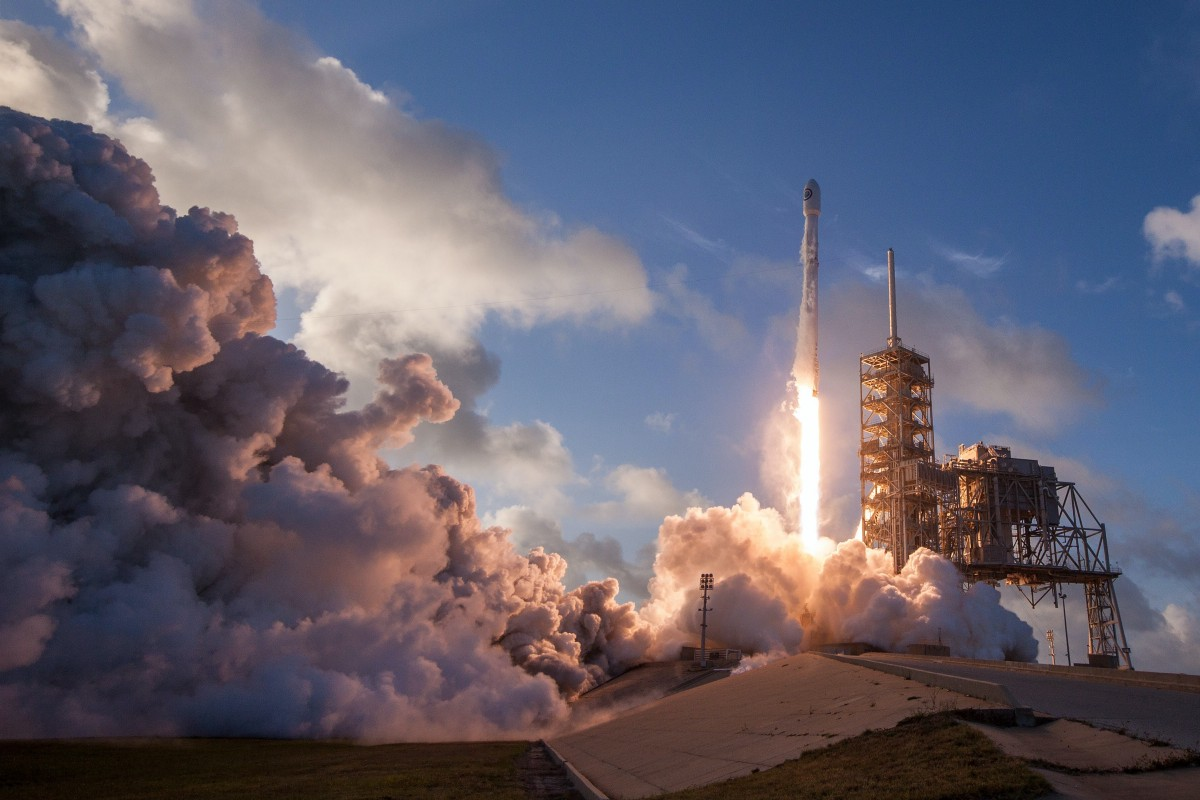
\includegraphics[width=3cm]{1 cyZbIB2epiZEV8A3xlm0Kg.jpeg}
    \caption{Rocket launch}
    \label{fig:my_label}
    \end{center}
\end{wrapfigure}
Lorem ipsum dolor sit amet, consectetur adipiscing elit, sed do eiusmod tempor incididunt ut labore et dolore magna aliqua. Ut enim ad minim veniam, quis nostrud exercitation ullamco laboris nisi ut aliquip ex ea commodo consequat. Duis aute irure dolor in reprehenderit in voluptate velit esse cillum dolore eu fugiat nulla pariatur. Excepteur sint occaecat cupidatat non proident, sunt in culpa qui officia deserunt mollit anim id est laborum. Lorem ipsum dolor sit amet, consectetur adipiscing elit, sed do eiusmod tempor incididunt ut labore et dolore magna aliqua. Ut enim ad minim veniam, quis nostrud exercitation ullamco laboris nisi ut aliquip ex ea commodo consequat. Duis aute irure dolor in reprehenderit in voluptate velit esse cillum dolore eu fugiat nulla pariatur. Excepteur sint occaecat cupidatat non proident, sunt in culpa qui officia deserunt mollit anim id est laborum. 

\section{Fifth session}

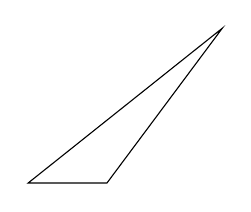
\begin{tikzpicture}
    \draw (1:2) -- (2:1) -- (30:4) -- cycle ;
\end{tikzpicture}

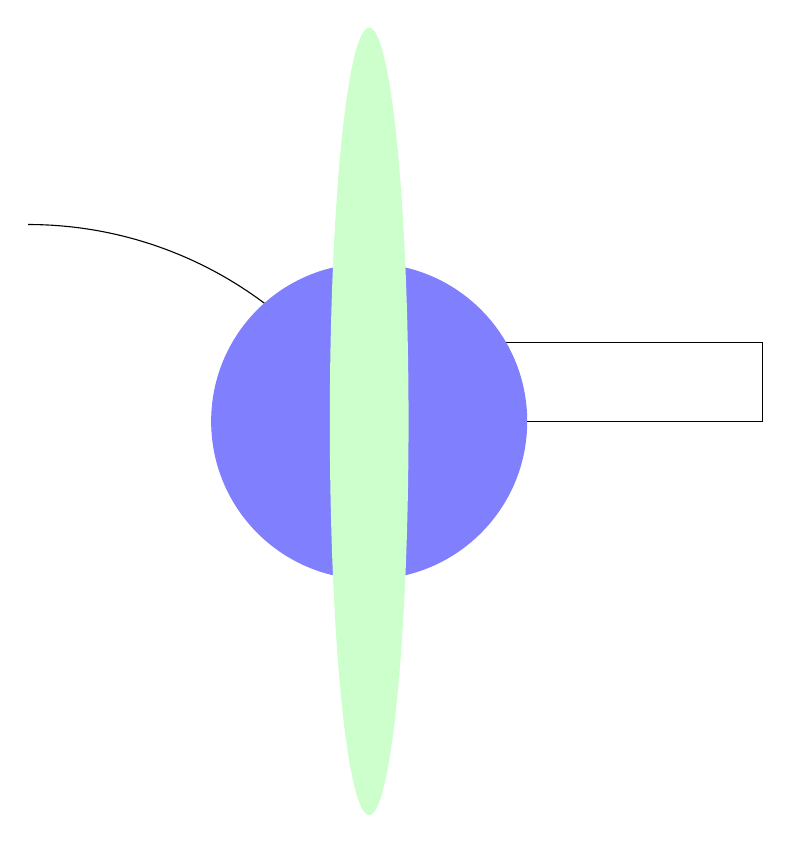
\begin{tikzpicture}
    \draw (0,0) arc [start angle = 30, end angle = 90, radius = 5cm];
    \draw (0,0) rectangle (5,1);
    \filldraw[blue!50] (0,0) circle [radius=2];
    \fill[green!20] (0,0) circle [x radius=0.5, y radius=5];
\end{tikzpicture}

\begin{tikzpicture}
    \draw[red,dashed,->] (0,0) ..controls (5,4) and (7,9).. (10,5);
\end{tikzpicture}

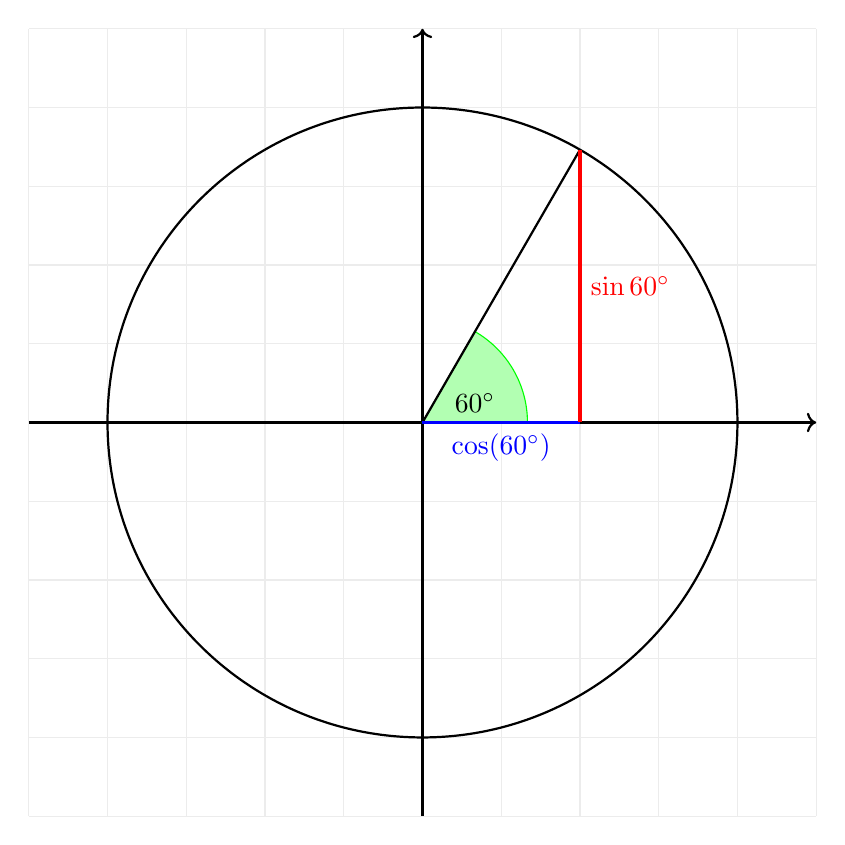
\begin{tikzpicture}
\colorlet{coscolor}{blue}
\colorlet{sincolor}{red}
\tikzset{anglefill/.style={draw=green,fill=green!30}}
\pgfmathsetmacro{\r}{4}
\pgfmathsetmacro{\a}{60}
\draw[lightgray!30] (-5,-5) grid[step=1] (5,5);
\draw[thick,->] (0,-5) -- (0,5);
\draw[thick,->] (-5,0) -- (5,0);
\filldraw[anglefill] (0,0) -- node[above]{$\a^\circ$}
(\r/3,0) arc [start angle=0,end angle=\a,radius=\r/3] -- cycle;
\draw[thick] (0,0) circle[radius=\r] -- (\a:\r);
\draw[very thick,coscolor] (0,0) --
node[below]{$\cos(\a^\circ)$} (\r*cos{\a},0);
\draw[very thick,sincolor] (\r*cos{\a},0) --
node[right]{$\sin\a^\circ$}(\a:\r);
\end{tikzpicture}

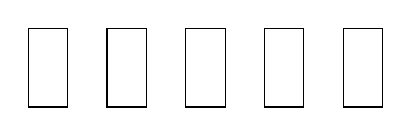
\begin{tikzpicture}
    \foreach \i in {1,2,3,4,5}{\draw (\i,0) rectangle (\i+0.5,1);}
\end{tikzpicture}

\medskip
\begin{tikzcd}
    X \arrow[r,dashed,"f"] & Y 
\end{tikzcd}

\begin{tikzcd}
    A \arrow[r,bend right,"\pi^2"] & B \arrow[r,bend left,tail] & C
\end{tikzcd}

\begin{tikzcd}
    A  \arrow[d,"1"'] \arrow[dr,"2"] & B \\ C & D \arrow[l] \arrow[u,out=45,in=0]
\end{tikzcd}

\begin{tikzcd}
    T \arrow[dr,dotted,"{(x,y)}" description] \arrow[drr,bend left, "x"] \arrow[ddr,bend right,"y"] & & \\ & X \arrow[r,"p"] \arrow[d,"q"] & X \arrow[d,"f"] \\ & Y \arrow[r,"g"] & Z
\end{tikzcd}

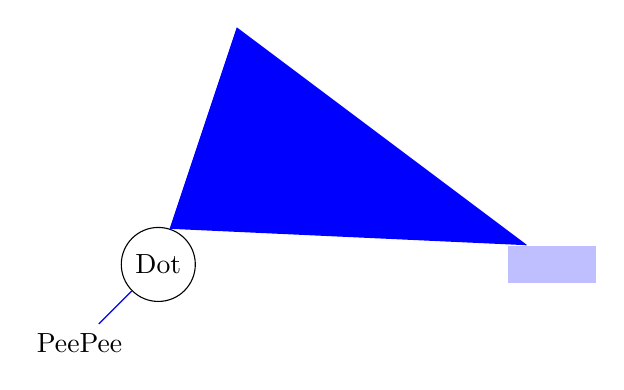
\begin{tikzpicture}
    \node (P) at (1,1) {PeePee};
    \node [draw, circle = 1pt] (Q) at (2,2) {Dot};
    \coordinate (R) at (3,5);
    \node [fill,blue!25, rectangle = 2pt] (S) at (7,2) {Seven};
    \filldraw [blue] (P) -- (Q) -- (R) -- (S) -- cycle;
\end{tikzpicture}


\begin{center}
    \schemestart
    \chemfig {C([:-30]=C ([::-60]-C ([::-60]=C ([::-60]-C()))))}
    \schemestop
\end{center}

\end{document}